\section{Desarrollo Frontend y Experiencia de Usuario (UX)}
\label{sec:frontend}

El ecosistema de interfaces de cliente se unificó bajo la nueva arquitectura del proyecto, dotando a la aplicación de un diseño interactivo, responsivo y orientado a la conversión.

\subsection{Gestión y Edición de Perfil}
Se desarrolló la vista principal de administración (\comando{/dashboard/profile}) donde se cargan dinámicamente los datos del usuario. Se incorporaron herramientas de validación estricta en tiempo real para formatos de texto y enlaces (URLs). El sistema previene el envío de formularios corruptos mediante bloqueos dinámicos en el botón de guardado y emite advertencias preventivas si el usuario intenta abandonar la vista con cambios no registrados.

\subsection{Componentes Dinámicos y Vistas Públicas}
Se implementaron formularios controlados (\comando{ExperienceForm}, \comando{EducationForm}) para la captura de trayectoria laboral y académica, dotados de validaciones cronológicas que impiden el registro de fechas de finalización anteriores al inicio. Estos datos alimentan el componente interactivo \comando{CareerTimeline}, el cual automatiza el cálculo de antigüedad. Las vistas públicas y privadas fueron acopladas exitosamente a la barra de navegación principal, integrando indicadores visuales de disponibilidad del profesional.

\subsection{Estrategia de Conversión de Usuarios Invitados}
La interfaz pública implementa estrategias visuales para fomentar la creación de cuentas \\(\comando{GuestProfileView}). Las redes sociales del profesional se enmascaran bajo íconos de acceso restringido y la línea de tiempo de experiencia recibe un efecto de desenfoque (\textit{blur}) escalonado. Un \textit{banner} persistente y un modal automático interactúan con el invitado para ejecutar el llamado a la acción de registro tras 30 segundos de inactividad.

\begin{BreakingChange}
El sistema de diseño adoptó \comando{Sora} como tipografía corporativa estándar. Todos los componentes renderizados deben heredar la directiva global configurada en los ficheros \comando{index.html} e \comando{index.css}.
\end{BreakingChange}

\subsection{Evidencia Visual y Flujos de Interfaz}
\label{ssec:evidencia_visual}

Como respaldo del avance funcional en la capa de cliente, se han consolidado las vistas correspondientes a la interacción principal del usuario. La implementación superó la fase de prototipado para convertirse en componentes interactivos completamente renderizados y enlazados al estado de la aplicación. 

Entre los flujos habilitados y evidenciados en este incremento se destacan:
\begin{itemize}
    \item \textbf{Página de Aterrizaje (Landing Page):} Despliegue del \textit{Hero Section} con la propuesta de valor de EthosHub, integrando navegación condicional en la cabecera según el estado de la sesión (botones de ingreso para invitados frente a menú de perfil para usuarios autenticados).
    \item \textbf{Módulo de Autenticación:} Formularios limpios para la creación de cuentas (\textit{Sign Up}), incluyendo validación de campos y la integración visual de los botones de inicio de sesión único (SSO) mediante GitHub y Google.
    \item \textbf{Flujo de Onboarding (Selección de Rol):} Pantallas de enrutamiento estratégico donde el usuario define el propósito de su cuenta, bifurcando la experiencia de configuración entre \comando{Cuenta profesional} y \comando{Cuenta reclutador}.
    \item \textbf{Formularios Dinámicos de Perfil:} Interfaces de configuración integral que abarcan la carga de fotografía, definición del estado de disponibilidad mediante selectores visuales, gestión de redes (LinkedIn, GitHub, Web) y los formularios modulares interactivos para la adición de trayectoria académica y laboral.
\end{itemize}

\begin{figure}[htbp]
    \centering
    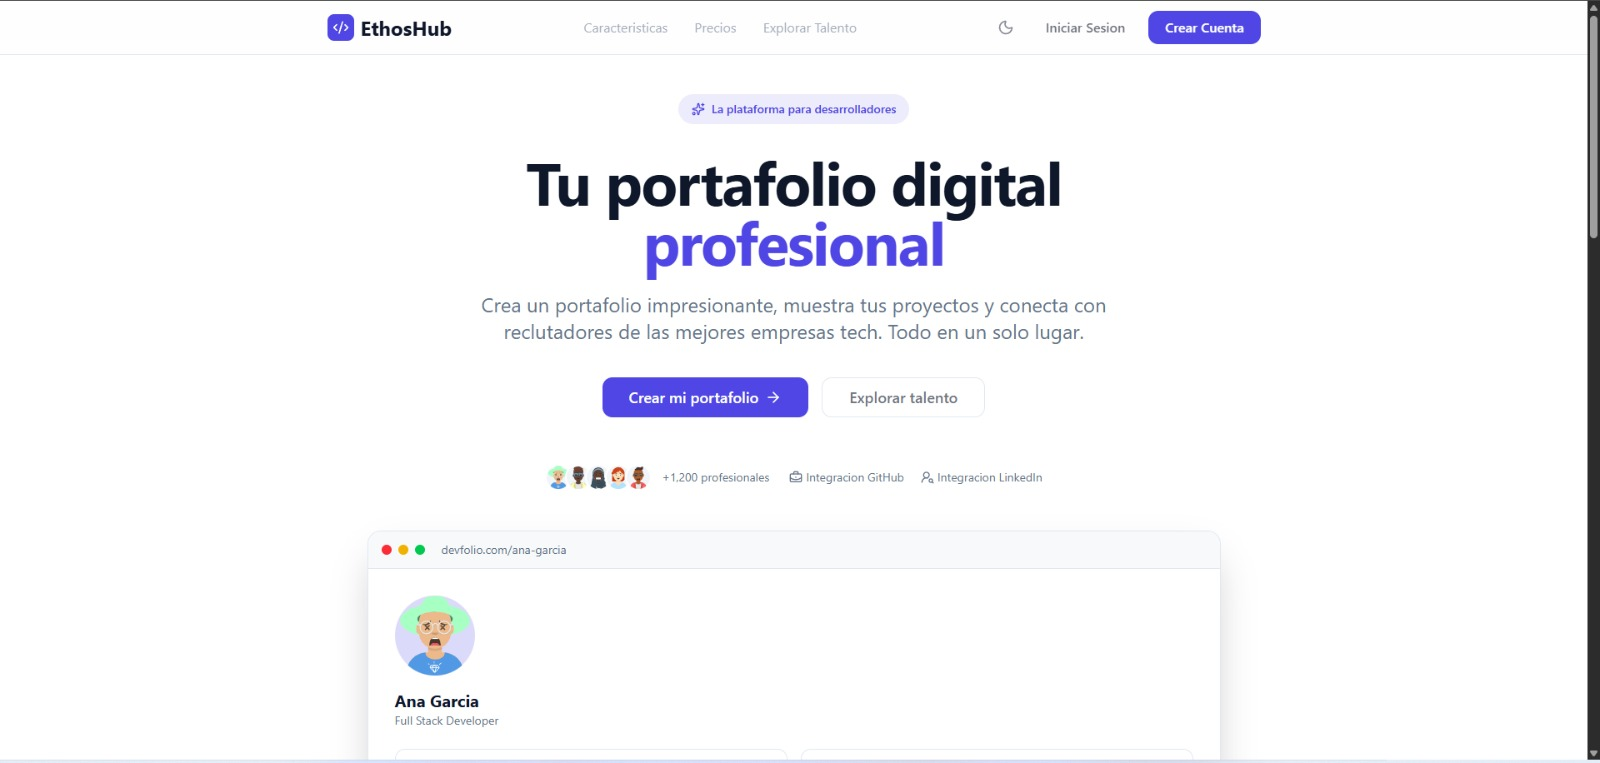
\includegraphics[width=0.7\textwidth]{assets/img/frontend/frontend7.jpeg}
    \caption{Despliegue de la página de aterrizaje (Landing Page) pública.}
    \label{fig:front_landing}
\end{figure}

\begin{figure}[htbp]
    \centering
    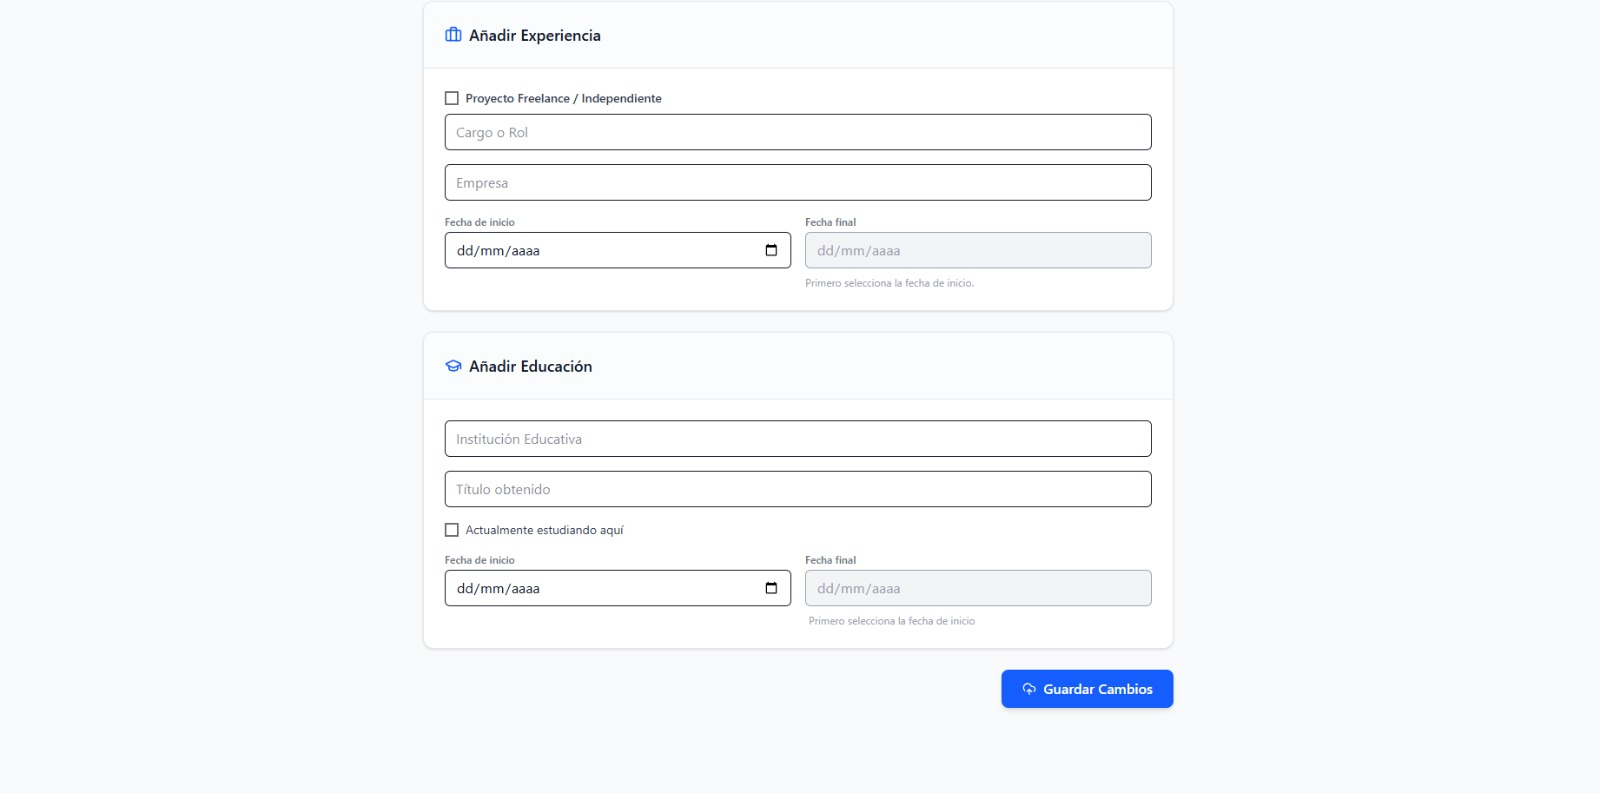
\includegraphics[width=0.7\textwidth]{assets/img/frontend/frontend5.jpeg}
    \caption{Componentes de formulario dinámico para la gestión de experiencia y educación, demostrando las validaciones cronológicas.}
    \label{fig:front_forms}
\end{figure}

\begin{figure}[htbp]
    \centering
    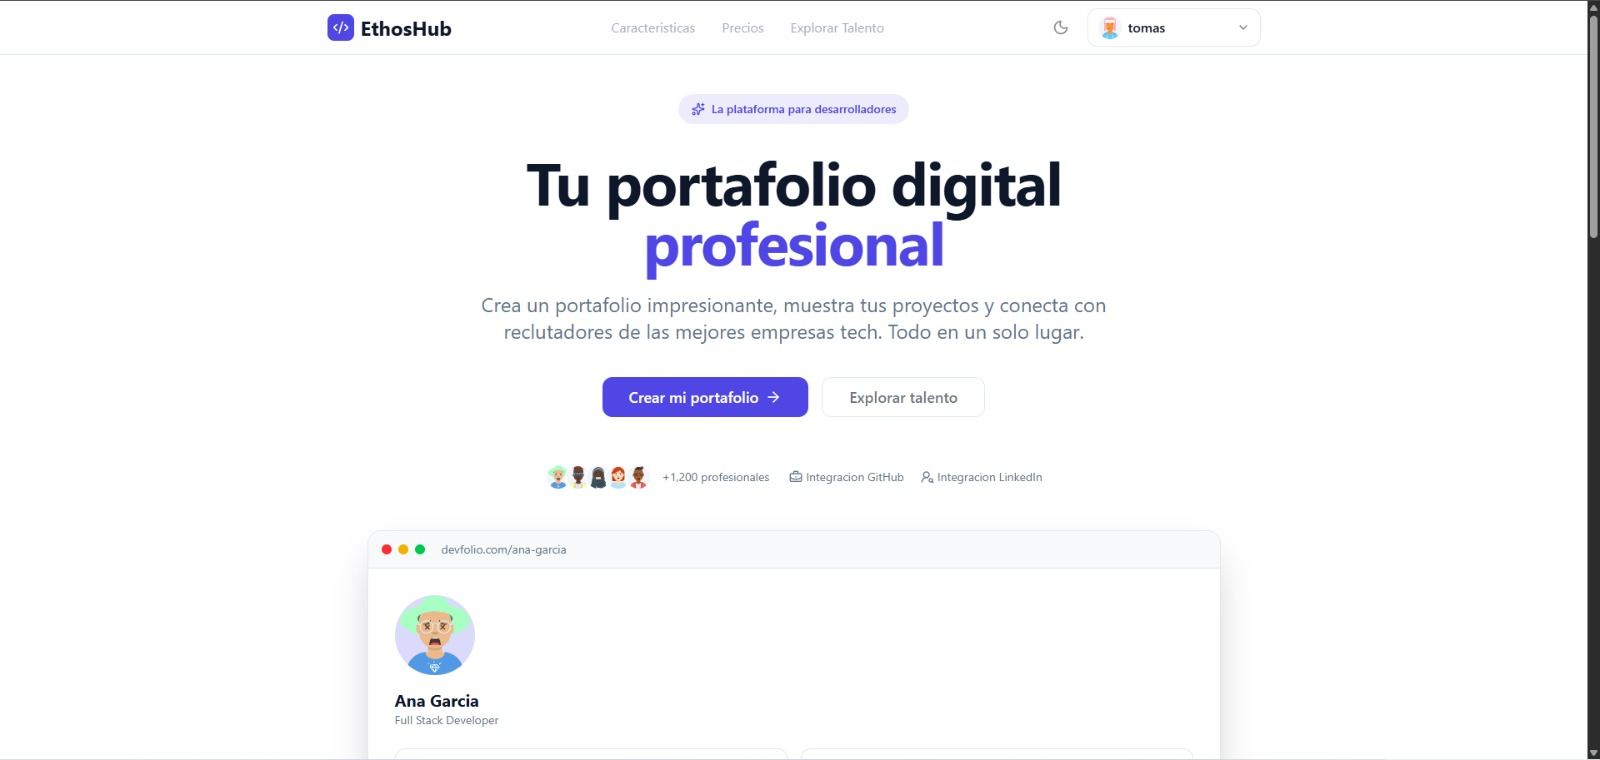
\includegraphics[width=0.7\textwidth]{assets/img/frontend/frontend8.jpeg}
    \caption{Página de aterrizaje en su vista autenticada. Se observa la adaptación dinámica de la barra de navegación, reemplazando los botones de ingreso por el menú desplegable del perfil del usuario en sesión.}
    \label{fig:front_landing_auth}
\end{figure}

\begin{figure}[htbp]
    \centering
    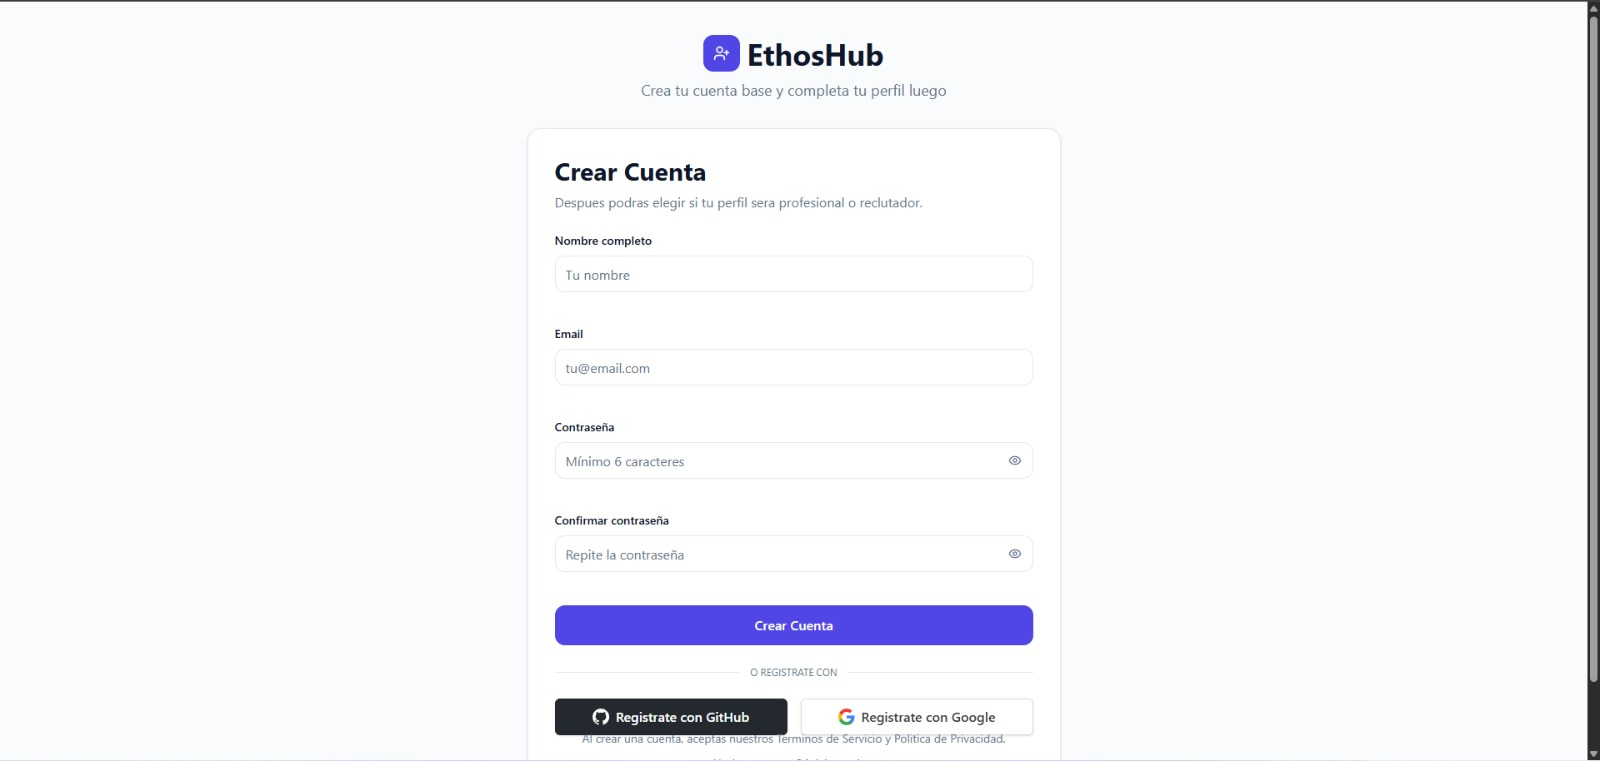
\includegraphics[width=0.7\textwidth]{assets/img/frontend/frontend6.jpeg}
    \caption{Interfaz de Registro de Cuenta (\textit{Sign Up}). Incluye validación de campos para correo y contraseña, y exhibe la integración de los flujos de autenticación OAuth2 (SSO) mediante GitHub y Google.}
    \label{fig:front_register}
\end{figure}

\begin{figure}[htbp]
    \centering
    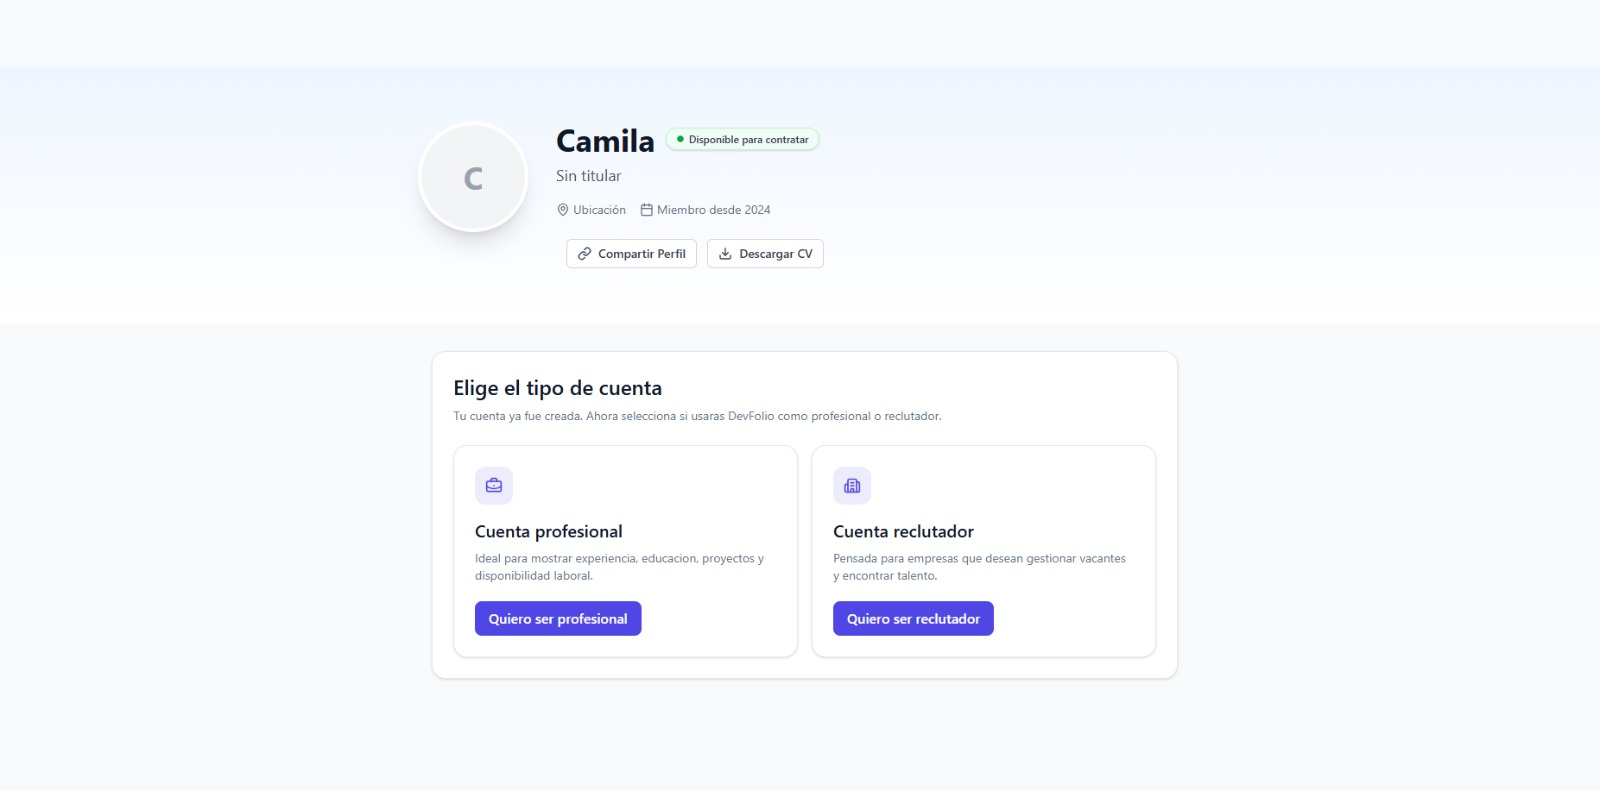
\includegraphics[width=0.7\textwidth]{assets/img/frontend/frontend1.jpeg}
    \caption{Flujo de Onboarding post-registro. Pantalla de selección de tipo de cuenta que bifurca la experiencia del usuario entre \comando{Cuenta profesional} y \comando{Cuenta reclutador}.}
    \label{fig:front_account_type}
\end{figure}

\begin{figure}[htbp]
    \centering
    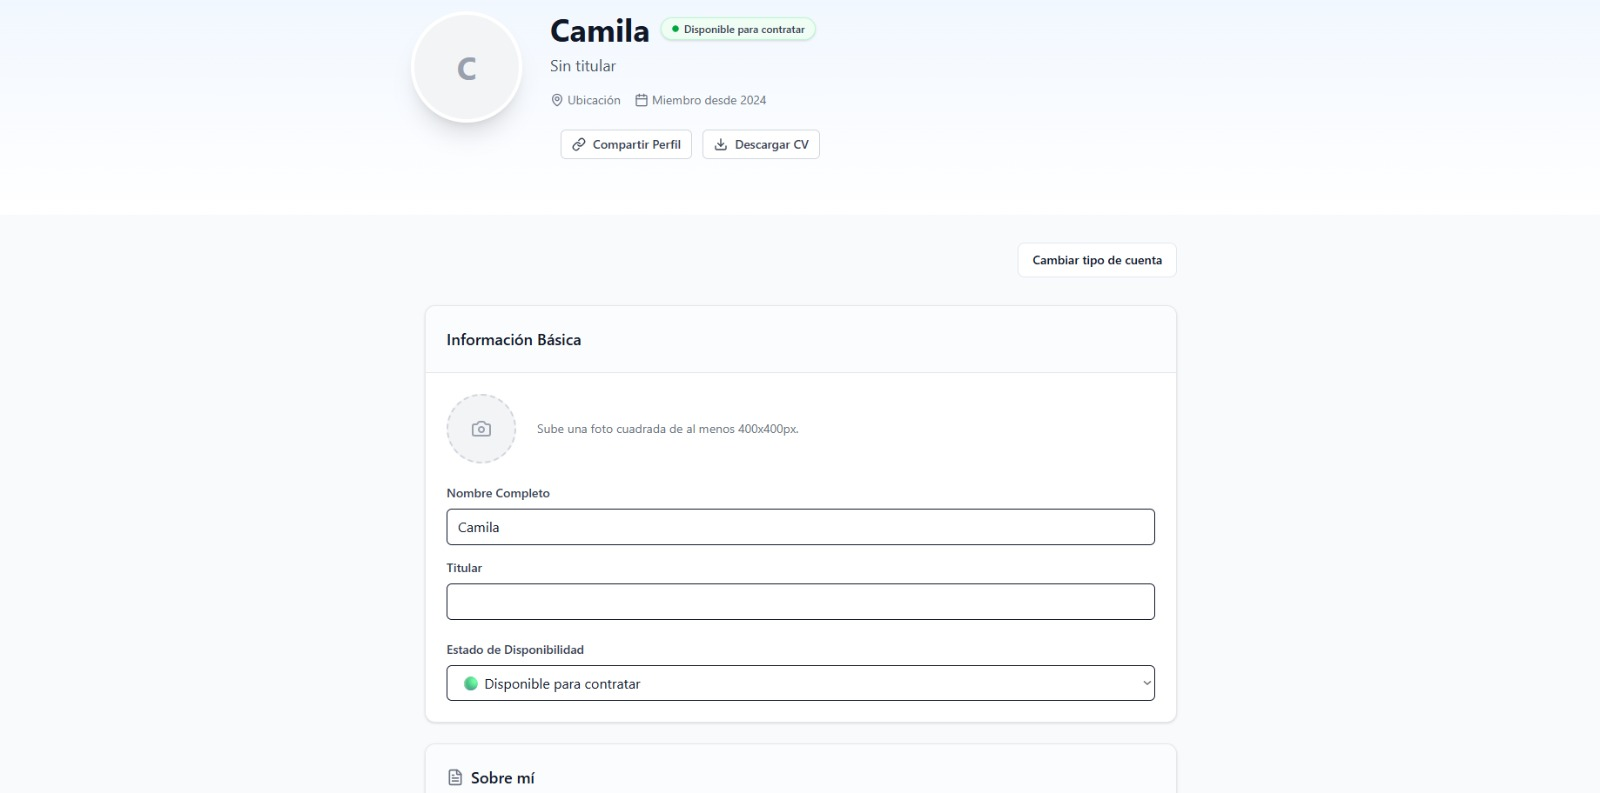
\includegraphics[width=0.7\textwidth]{assets/img/frontend/frontend2.jpeg}
    \caption{Módulo de configuración de Perfil Profesional (Parte 1). Formulario de Información Básica que permite la carga de fotografía, definición del nombre, titular profesional y la gestión del estado de disponibilidad mediante un selector visual.}
    \label{fig:front_basic_info}
\end{figure}

\begin{figure}[htbp]
    \centering
    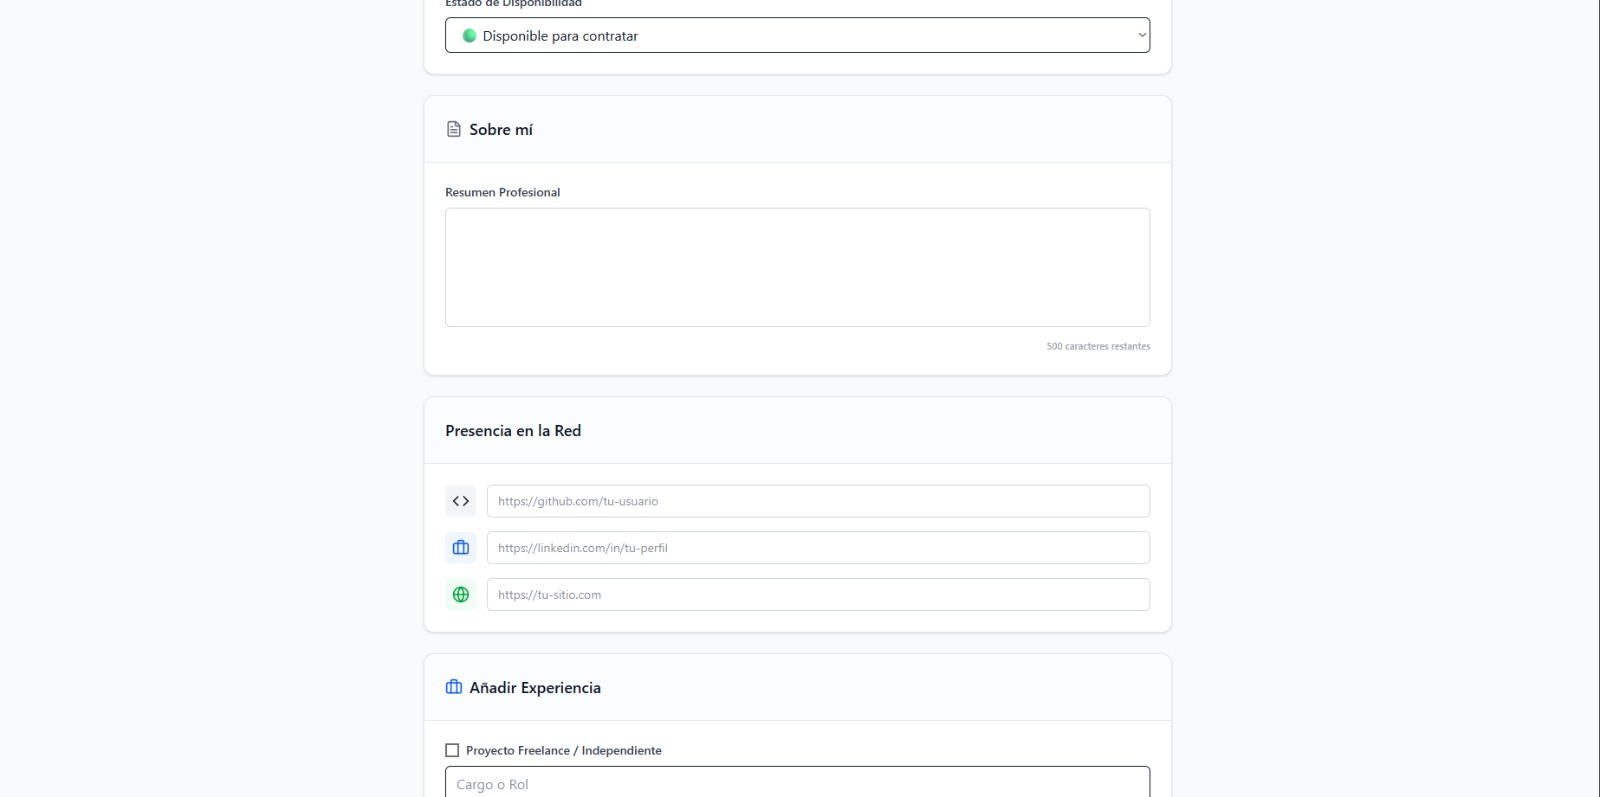
\includegraphics[width=0.7\textwidth]{assets/img/frontend/frontend4.jpeg}
    \caption{Módulo de configuración de Perfil Profesional (Parte 2). Secciones dedicadas a la biografía del usuario (\textit{Sobre mí}) y la parametrización de enlaces externos para su \textit{Presencia en la Red} (GitHub, LinkedIn, Sitio Web).}
    \label{fig:front_about_network}
\end{figure}

\begin{figure}[htbp]
    \centering
    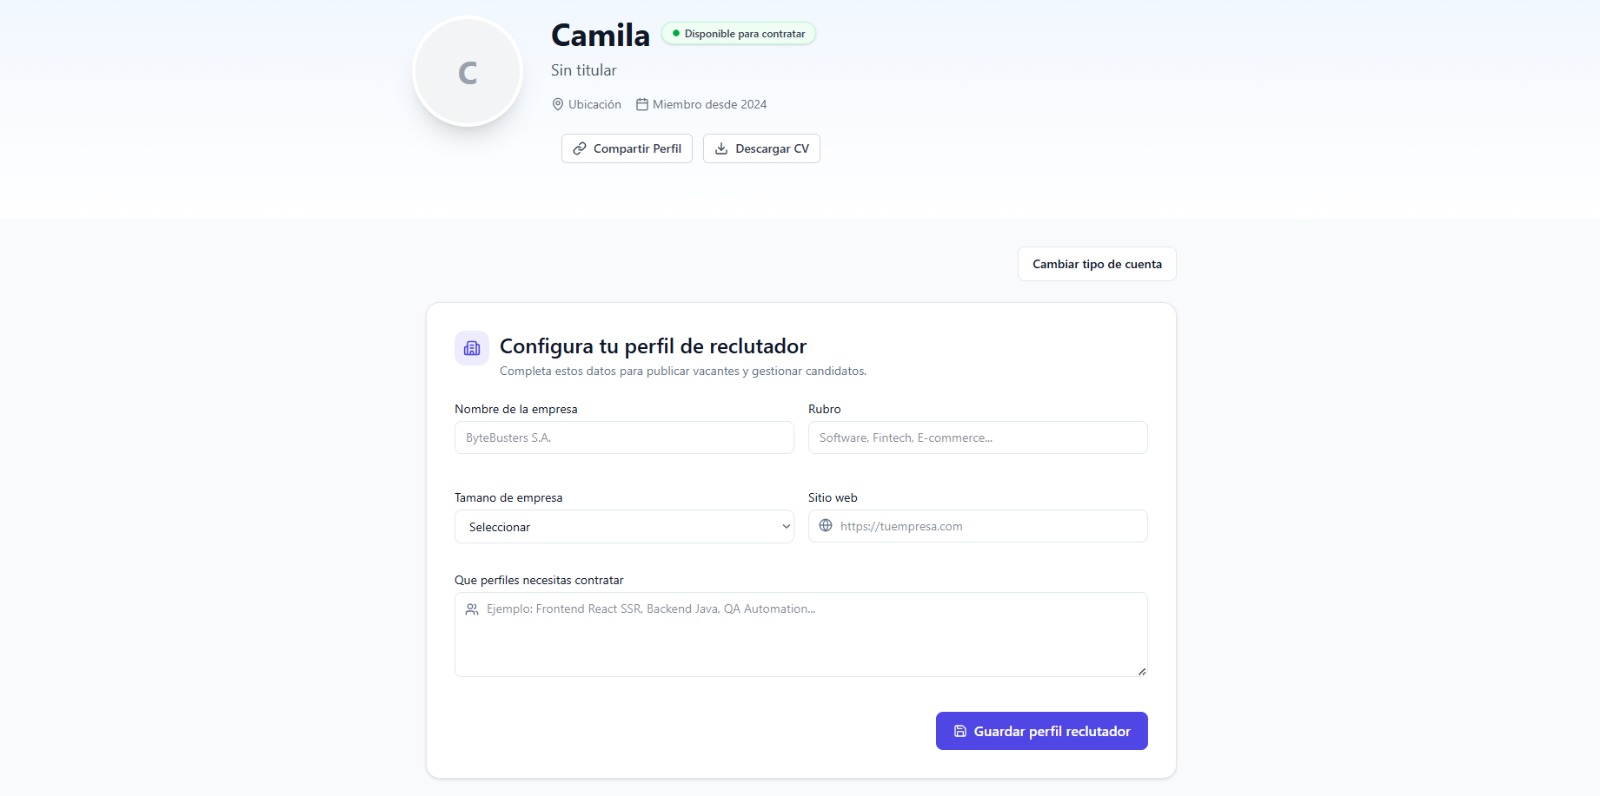
\includegraphics[width=0.7\textwidth]{assets/img/frontend/frontend3.jpeg}
    \caption{Interfaz de configuración para la \comando{Cuenta reclutador}. Permite a las empresas definir su rubro, tamaño, sitio web corporativo y detallar los perfiles tecnológicos que necesitan contratar.}
    \label{fig:front_recruiter}
\end{figure}

\begin{NotaTecnica}
Las interfaces desarrolladas demuestran la correcta aplicación de la tipografía global \comando{Sora} y el respeto estricto por la jerarquía visual de los \textit{mockups} originales, cumpliendo con los criterios de aceptación de usabilidad y diseño responsivo establecidos para el Sprint.
\end{NotaTecnica}